In the regular approach to the explore-exploit dilemma decisions are understood in terms of reward. For example, if a bee goes to a familiar direction \textit{to gather nectar}, it is said to be exploiting past knowledge. If it goes in an unknown direction \textit{to gather nectar}, it is said to be exploring. Because the environment seems stochastic to the bee it cannot know if it should be exploiting or exploring \textit{to gain more nectar}. It is this uncertainty \textit{about rewards} that makes the choice a real dilemma, with no tractable mathematical solution \citep{Thrun1992a,Dayan1996,Ishii2002,Simsek2006,Gershman2018b}. We illustrate this in Fig. \ref{fig:bee}a. 

This dilemma is faced routinely by learners of all kinds, including by foraging bees, business organizations, humans, worms, monkeys, rodents, birds, children, and computer algorithms \citep{Gupta2006,Sutton2018,Woodgate2017,Lee2011a,Schulz2018a,Calhoun2014,Wang2019,Sumner2019,Auersperg2015}. But is reward fundamental to the problem? 

In the natural world exploration finds two explanations. If there is no reason to expect a reward, exploration is described theoretically as a search for information, what we will call curiosity \citep{Berlyne1950,Schmidhuber1991,Kidd2015,deAbril2018,Jaegle2019,Friston2016}. On the other hand, if reward is expected exploration gets re-interpreted as a search for that reward, which is what leads to the dilemma \citep{Kelly1956,Berger-Tal2014,Dayan1996,Thrun1992,Mehlhorn2015,Kobayashi2019}. We argue here that all exploration should be treated as a curiosity search. We illustrate this in Fig. \ref{fig:bee}b.

\begin{figure}
	\begin{fullwidth}
	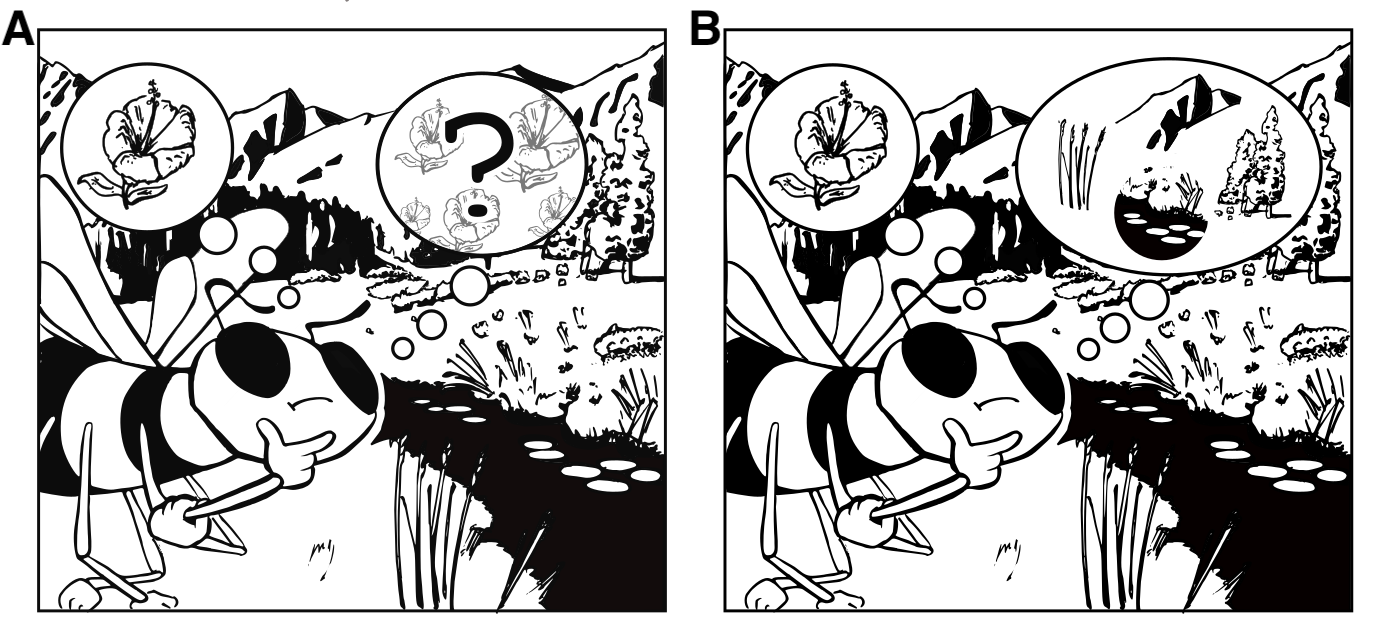
\includegraphics[width=.5\linewidth]{figures/fig1.png} 
	\caption{Two views of exploration and exploitation. \textbf{a}. The classic dilemma: either exploit an action with a known reward (e.g., return to the previous flower) or explore other actions on the chance they will return a better outcome. The central challenge here is that the outcome of exploration is uncertain, and filled with questions. \textbf{b}. An alternative view of the dilemma, with two goals: either maximize rewards \textit{or} maximize information value with a curious search of the environment. \textit{Artist credit}: Richard Grant.}
	\label{fig:bee} 
	\end{fullwidth}
\end{figure}

The first half of this paper is devoted to developing a new view of curiosity, that can span all fields. This is, it turns out, the same formal problem as learning to value information. We then develop proofs for what we can expect from any curious search. The second half will use the first results to prove curiosity can eliminate this dilemma, if two conjectures we make are true.

% Our contribution is threefold. We offer a new measure of information value. We use this as an objective for curiosity, and prove the computer science method of dynamic programming \citep{Bellmann1954,Roughgarden2019} will maximize any curious search. Finally, we derive a solution to the dilemma based on curiosity. We also in this work introduce a new use for boredom.

